\chapter{Contenido multimedia y streaming}\label{chap:5}
\section{Vídeo en la web}
\subsection{Ejercicio 1}
Una vez creado el \Verb#index.html#, se lanza la imagen de docker mediante el
siguiente comando:
\begin{verbatim}
docker run --rm -d --network pruebas --name nginx -p 80:80
    -v $(pwd)/html/video5/:/usr/share/nginx/html nginx
\end{verbatim}

Al acceder a \Verb#localhost:80#, se accede correctamente a la página web: \\
\begin{minipage}{\linewidth}
	\centering
	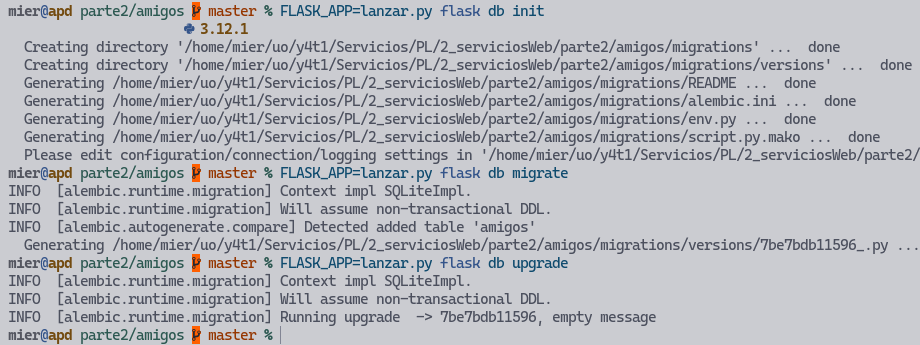
\includegraphics[width=0.8\textwidth]{5/1.png}
	\captionof{figure}{Página web con el vídeo}\label{fig:5/1}
\end{minipage}

Mediante las herramientas de desarrollador, se aprecia que se descargan fragmentos del vídeo
según se necesiten, incluyendo las cabeceras que especifican el rango de bytes a descargar: \\
\begin{minipage}{\linewidth}
	\centering
	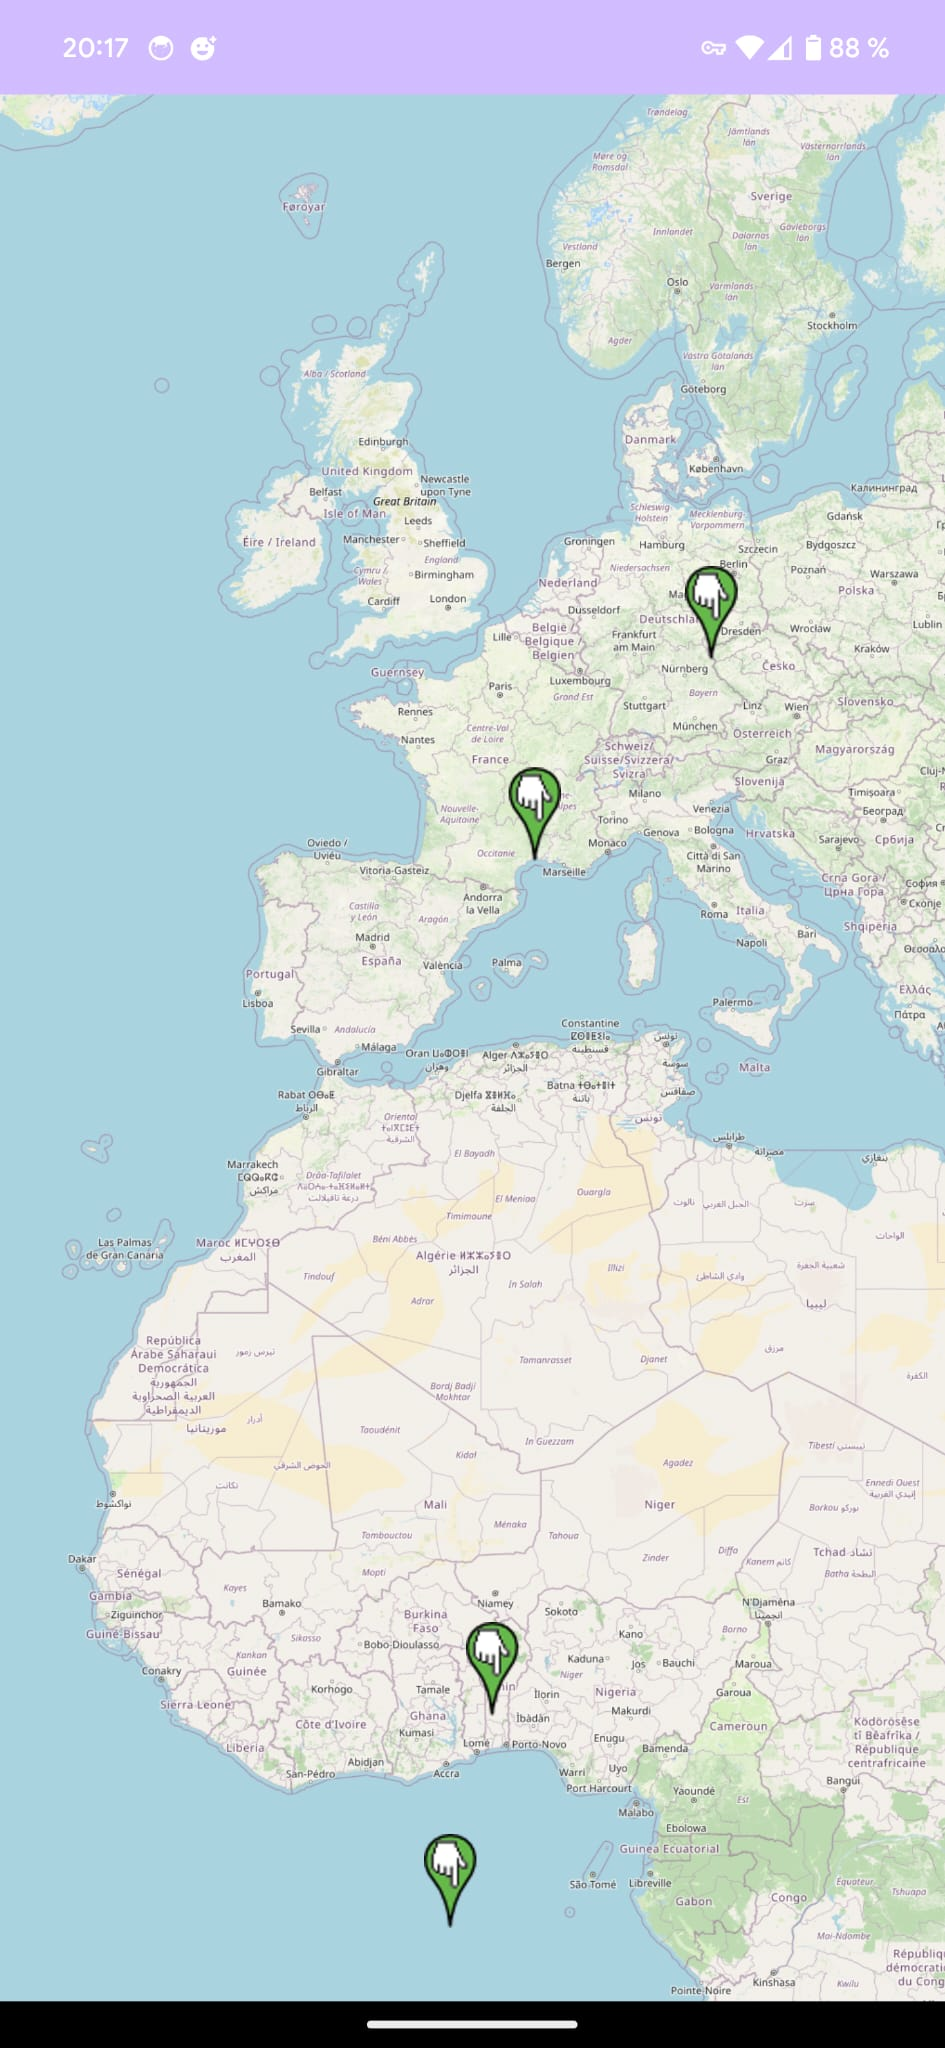
\includegraphics[width=0.8\textwidth]{5/2.png}
	\captionof{figure}{Cabeceras de la descarga del vídeo}\label{fig:5/2}
\end{minipage}

\subsubsection{Modifica ahora la página y utiliza como fuente otro vídeo}
En mi caso, Firefox en Linux admite los tres formatos disponibles (\Verb#mp4#, \Verb#webm# y \Verb#ogv#).
|TODO| revisar

\subsubsection{Modifica la página anterior para incluir todas las fuentes disponibles}
Este ejercicio no tiene más gracia que añadir las tres fuentes disponibles en la página web,
una detrás de otra junto con un mensaje de error en caso de que no se pueda reproducir el vídeo.

\begin{verbatim}
...
<source ... type="video/ogg;  codecs...">
<source ... type="video/mp4;  codecs...">
<source ... type="video/webm; codecs...">

<object type="application/x-shockwave-flash" ...>
	...
	<!-- Fallback final: -->
	<p>No se puede reproducir el video</p>
</object>
...
\end{verbatim}

\subsection{Ejercicio 2.~videojs}

\section{Servidor de streaming}
